\documentclass[a4paper]{amsart}
\usepackage{a4wide}
\usepackage[]{graphicx}

\setlength{\parindent}{0.0in}
\setlength{\parskip}{0.1in}

\newcommand{\laplace}[1]{\mathcal{L}\{#1\}}
\newcommand{\Hv}{\textrm{H}}
\renewcommand{\b}{\mathbf}

\begin{document}
\title{6G5Z3011 Multi-variable calculus and analytical methods}
\author{Tutorial Sheet 8}
\maketitle

\textbf{Qs 1 -- 4} on working with the Heaviside step function and Dirac delta function. \\
\textbf{Qs 5 -- 9} on transforms of Heaviside step function and Dirac delta function and solving ODEs featuring them.

\begin{enumerate}
    \item
Sketch each of the following functions and express them in terms of Heaviside functions.
\begin{enumerate}
    \item
    $$
       f(t) = \left\{
         \begin{array}{lr}
           6, &  2 < t \leq 3\\
           0, & \text{elsewhere} 
         \end{array}
       \right.
    $$
    \item
    $$
       f(t) = \left\{
         \begin{array}{lr}
           0, &  t \leq 1 \\
           t-1, & t > 1 
         \end{array}
       \right.
    $$
    \item
    $$
       f(t) = \left\{
         \begin{array}{lr}
           0, &  t \leq 2\\
           t-2, & 2 < t \leq 6 \\
           4, & t > 6 
         \end{array}
       \right.
    $$
    \item
    $$
       f(t) = \left\{
         \begin{array}{lr}
           3t, &  0 < t \leq 1\\
           4-t, & 1< t \leq 4 \\
           0, & t > 4 
         \end{array}
       \right.
    $$
    \end{enumerate}
    \item
    Express the function correspoding to the graph below in terms of Heaviside functions.
    \begin{center}
    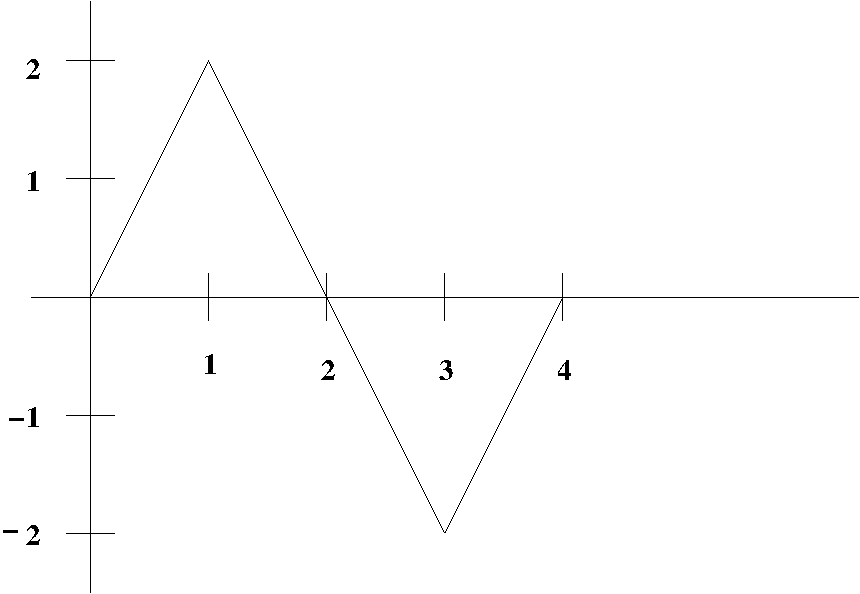
\includegraphics[scale=0.5]{sheet3q2.pdf} 
    \end{center}
    \item
    Sketch graphs of the following functions.
    \begin{enumerate}
    \item
    $\Hv(t) - \Hv(t-3)$
    \item
    $ t \left ( \Hv(t-2) - \Hv(t-4) \right ) $
    \item
    $\delta(t) + t^2 \Hv(t) - (t^2 - 4) \Hv(t-2) - 4\Hv(t-4) + \delta(t-4)$
    \end{enumerate}
    \item
    Prove that if $F(s)$ is the Laplace transform of the function $f(t)$ then the transform $f(t-a)\Hv(t-a)$ is $e^{-as} F(s)$.


    %%%%%%%%%%%%%%%%%%%%%%%%%

    \item
Find the Laplace transform of the following functions.
\begin{enumerate}
\item
$3 \delta(t-1) + 4 \Hv(t+2)$
\item
$t \Hv(t-4)$
\item
$\cos{(t-3)} \Hv(t-3)$
\item
$t^2 \Hv(t-1)$
\end{enumerate}
\item
Find the inverse Laplace transform of the following functions
\begin{enumerate}
\item
$2 e^{-4s} + 5 \dfrac{e^{-5s}}{s}$
\item
$\left ( \frac{3}{s+4} + \frac{s}{s^2 +1} \right ) e^{-s}$
\end{enumerate}
\item
\begin{enumerate}
\item
Solve the following differential equations subject, in both cases, to the intial conditions $y(0)=y'(0)=0$.
\begin{enumerate}
\item
$$\frac{d^2y}{dt^2} - 6 \frac{dy}{dt} + 5y = 4 \delta(t-2)$$
\item
$$ \frac{d^2y}{dt^2} + 4 \frac{dy}{dt} + 3y = (t-1) \Hv(t-1)$$
\end{enumerate}
\item
Given the intial condition $y(0)=0$ solve the differential equation
$$ \frac{dy}{dt} - y = f(t),$$
where $f$ is the function defined by 
$$
   f(t) = \left\{
     \begin{array}{lr}
       t, &  0 < t \leq 1\\
       1, & 1 < t \leq 2 \\
       3-t, & 2 < t \leq 3 \\
       0, & \text{elsewhere} 
     \end{array}
   \right. .
$$
\end{enumerate}
\item
Find the inverse Laplace transforms of the functions given by the following expressions. Identify the steaty state and transient parts of the function and show that in each case the initial and final value theorems hold.
\begin{enumerate}
\item
$$\dfrac{4}{s+2} + \dfrac{7}{s-3} $$
\item
$$\dfrac{5s+17}{s^2 + 6s +10}$$
\item
$$\dfrac{25+14s}{s^2 + 6s + 8} e^{-s}$$
\end{enumerate}
\item
Solve the differential eqaution
$$\frac{d^2y}{dt^2} + 6 \frac{dy}{dt} + 8y = 16$$ 
subject to the intial conditions $y(0)=3$ and $y'(0)=4$. Identify the steady state and transient parts of the solution. Verify that the intial and final value theorems hold for the transform of $y$.
\end{enumerate}

\end{document}